% OpenJaw Part I: Architecture and Mathematical Framework for RL-Based
% Visual-Acoustic Articulatory Speech Imitation
% Targeting NeurIPS / ICML / ICLR format

\documentclass[11pt, a4paper]{article}

% Use standard packages (compatible with BasicTeX)
% To switch to NeurIPS format: replace these lines with \usepackage[final]{neurips_2024}
\usepackage[margin=1in]{geometry}

\usepackage[utf8]{inputenc}
\usepackage[T1]{fontenc}
\usepackage{hyperref}
\usepackage{url}
\usepackage{booktabs}
\usepackage{amsfonts}
\usepackage{amsmath}
\usepackage{amssymb}
\usepackage{graphicx}
\usepackage{subcaption}
\usepackage{algorithm}
\usepackage{algorithmic}
\usepackage{multirow}
\usepackage{xcolor}
\usepackage{natbib}

\newcommand{\R}{\mathbb{R}}
\newcommand{\E}{\mathbb{E}}
\newcommand{\openjaw}{\textsc{OpenJaw}}
\newcommand{\sparc}{\textsc{SPARC}}
\newcommand{\sylber}{\textsc{Sylber}}
\newcommand{\mujoco}{\textsc{MuJoCo}}
\newcommand{\flame}{\textsc{FLAME}}

\title{\openjaw{} Part~I: Architecture and Mathematical Framework\\for RL-Based Visual-Acoustic Articulatory Speech Imitation}

\author{\large White Paper}

\begin{document}

\maketitle

% ============================================================================
\begin{abstract}
We present \openjaw{}, a unified mathematical framework for closed-loop reinforcement learning (RL)-based embodied speech imitation. This paper (Part~I) establishes the architecture and mathematical foundations: (1)~a 13-DOF articulatory motor control problem formalized as a Markov Decision Process in a multi-physics oral cavity simulation (\mujoco{}); (2)~dual-modality output via a neural articulatory-to-audio decoder (\sparc{}) and mesh-based visual rendering; (3)~a multi-modal reward combining syllabic audio similarity (\sylber{}) and lip vertex error; and (4)~a custom PPO training loop with observation normalization, reward normalization, value function clipping, KL-based early stopping, and learning rate decay. We validate the framework through 10,000-episode training runs demonstrating stable policy optimization under the full 4-phase curriculum (babbling $\to$ vowels $\to$ syllables $\to$ person-specific). The agent successfully learns the babbling phase (reward $+40$) within 5 rollouts, with the critic achieving 0.50 explained variance. We provide rigorous ablation analysis of architectural components and release the full codebase with 229 passing tests. Part~II will integrate real SPARC and Sylber encoders for acoustic quality evaluation.
\end{abstract}

% ============================================================================
\section{Introduction}
\label{sec:introduction}

Human speech production is a remarkably complex sensorimotor skill: the brain coordinates over 70 muscles to produce rapid, precise movements of the tongue, jaw, lips, and larynx---generating both an acoustic signal and visible facial motion simultaneously~\cite{maeda2004compensatory}. Despite the central role of this motor control problem in speech science, computational approaches to articulatory synthesis have largely remained decoupled: audio-driven talking head models~\cite{richard2021selftalk, fan2022faceformer, xing2023codetalker} generate realistic facial motion but bypass the underlying physics, while biomechanical simulators~\cite{freeman2023artisynth, tian2019vocaltractlab} model the physics but lack the closed-loop learning necessary for autonomous speech acquisition.

Recent advances in deep reinforcement learning for continuous control~\cite{schulman2017ppo, haarnoja2018sac}, high-speed physics simulation~\cite{todorov2012mujoco}, and neural articulatory-to-audio decoding~\cite{parrot2024sparc} now make it feasible to bridge this gap. Anand et al.~\cite{anand2025articulatory} demonstrated that an RL agent can learn syllable-level articulatory control via direct optimization in the \sparc{} decoder space---but without physics simulation, visual output, or visual feedback.

We introduce \openjaw{}, the first unified mathematical framework that jointly models:
\begin{itemize}
    \item \textbf{RL-driven articulatory motor control} with 13 degrees of freedom in a \mujoco{} multi-physics simulation
    \item \textbf{Dual-modality output}: acoustic (via \sparc{} neural decoding) and visual (via mesh rendering)
    \item \textbf{Dual-modality reward}: audio similarity (\sylber{} cosine similarity) and visual fidelity (lip vertex error)
    \item \textbf{Closed-loop sensory feedback} for progressive policy improvement via curriculum learning
\end{itemize}

This paper (Part~I) focuses on the \emph{architecture, mathematical framework, and training methodology}. We validate the complete training pipeline using mock encoder components, demonstrating that the PPO loop converges under curriculum learning, the policy network learns meaningful behavior, and the training infrastructure (checkpointing, reward normalization, observation normalization) functions correctly at scale. Part~II will integrate real SPARC and Sylber encoders for acoustic quality evaluation.

Our contributions are:
\begin{enumerate}
    \item A \textbf{complete MDP formalization} for visual-acoustic articulatory imitation, including state/action/observation/reward spaces with exact dimensionalities and biomechanical grounding (Section~\ref{sec:mdp}).
    \item A \textbf{modular neural architecture} comprising a sub-million parameter actor-critic, frozen perception encoders, and a configurable multi-modal reward---designed for consumer GPU training (Section~\ref{sec:architecture}).
    \item A \textbf{custom PPO training loop} with 8 stability mechanisms validated through progressive ablation (Section~\ref{sec:training_stability}).
    \item \textbf{Framework validation} through 10,000-episode training runs demonstrating stable optimization under curriculum transitions, with 229 automated tests ensuring correctness (Section~\ref{sec:experiments}).
    \item \textbf{Rigorous methods analysis} justifying 7 critical design decisions through quantitative comparison of alternatives (Section~\ref{sec:methods_analysis}).
\end{enumerate}

% ============================================================================
\section{Related Work}
\label{sec:related_work}

\paragraph{Audio-driven talking heads.}
SelfTalk~\cite{richard2021selftalk}, FaceFormer~\cite{fan2022faceformer}, and CodeTalker~\cite{xing2023codetalker} produce high-quality 3D facial animation from audio using the VOCASET benchmark~\cite{li2021vocaset} and \flame{} topology~\cite{li2017flame}. These methods regress from audio features to vertex displacements via transformers or VAEs, but do not model the underlying articulatory physics---motion is an output, not the result of physical simulation.

\paragraph{Biomechanical articulatory simulation.}
ArtiSynth~\cite{freeman2023artisynth} provides a detailed finite-element model of the vocal tract with muscle-driven tongue, jaw, and lip control. VocalTractLab~\cite{tian2019vocaltractlab} uses a geometric tube model for real-time articulatory synthesis. Both achieve high physical fidelity but are computationally expensive (1--500 Hz simulation rate), making them impractical for RL training which requires millions of environment interactions.

\paragraph{RL for articulatory control.}
Anand et al.~\cite{anand2025articulatory} is the most directly related work: they train a PPO agent to control 13 articulatory parameters via the \sparc{} decoder, achieving $>$0.85 cosine similarity on 6 syllables. However, their approach operates directly in \sparc{}'s parameter space without physics simulation, produces no visual output, and does not use visual feedback for training. \openjaw{} extends this by embedding the control problem in a multi-physics simulation with dual-modality output and reward.

\paragraph{Self-supervised speech representations.}
wav2vec 2.0~\cite{baevski2020wav2vec} provides frame-level speech features suitable for observation construction. \sylber{}~\cite{cho2024sylber} extracts syllable-level embeddings from raw audio, enabling phonetically meaningful reward computation without explicit phoneme transcription.

% ============================================================================
\section{Methods}
\label{sec:methods}

\subsection{Problem Formulation}
\label{sec:problem}

We formalize articulatory speech imitation as a goal-conditioned RL problem. Given a reference speech signal $\mathbf{y}^* = (y^*_{\text{audio}}, y^*_{\text{visual}})$, the agent must learn a policy $\pi_\theta$ that controls a simulated oral cavity to produce output $\hat{\mathbf{y}} = (\hat{y}_{\text{audio}}, \hat{y}_{\text{visual}})$ that matches the reference in both acoustic and visual modalities.

\subsection{Markov Decision Process}
\label{sec:mdp}

We define the MDP $\mathcal{M} = (\mathcal{S}, \mathcal{A}, \mathcal{O}, T, R, \gamma, H)$:

\paragraph{State space.} $\mathcal{S} \subset \R^{39}$, where:
\begin{equation}
    \mathbf{s}_t = [\mathbf{q}_t, \dot{\mathbf{q}}_t, \mathbf{a}_{t-1}] \in \R^{13 + 13 + 13}
\end{equation}
with joint positions $\mathbf{q}_t \in \R^{13}$, velocities $\dot{\mathbf{q}}_t \in \R^{13}$, and previous action $\mathbf{a}_{t-1} \in \R^{13}$.

\paragraph{Action space.} $\mathcal{A} = [-0.5, 0.5]^{13}$, representing velocity commands for 13 articulatory degrees of freedom (Table~\ref{tab:dof}).

\paragraph{Observation space.} The agent observes a frame-stacked history and a target embedding:
\begin{equation}
    \mathbf{o}_t = [\mathbf{s}_{t-K+1}, \ldots, \mathbf{s}_t, \mathbf{e}^*] \in \R^{K \cdot 39 + d_e}
\end{equation}
where $K = 15$ frames provide temporal context and $\mathbf{e}^* \in \R^{768}$ is the \sylber{} embedding of the target syllable. Total observation dimension: $15 \times 39 + 768 = 1353$.

\paragraph{Transition dynamics.} $T(\mathbf{s}_{t+1} | \mathbf{s}_t, \mathbf{a}_t)$ is defined by the \mujoco{} physics engine with 20 substeps per control step at 25~Hz control frequency, yielding 500~Hz physics simulation.

\paragraph{Reward function.} (Section~\ref{sec:reward})

\paragraph{Episode structure.} Horizon $H = 50$ steps (2 seconds of speech), discount $\gamma = 0.99$, episode starts from neutral articulatory pose.

\begin{table}[t]
\centering
\caption{13-DOF articulatory action space following Anand et al.~\cite{anand2025articulatory}. Each DOF controls a velocity command within $[-0.5, 0.5]$.}
\label{tab:dof}
\small
\begin{tabular}{clll}
\toprule
DOF & Articulator & Parameter & Body Part \\
\midrule
1--2 & Tongue Dorsum & X, Y & Tongue \\
3--4 & Tongue Blade & X, Y & Tongue \\
5--6 & Tongue Tip & X, Y & Tongue \\
7--8 & Lower Incisor (Jaw) & X, Y & Jaw \\
9--10 & Upper Lip & X, Y & Lips \\
11--12 & Lower Lip & X, Y & Lips \\
13 & Vocal Loudness & Scalar & Voicing \\
\bottomrule
\end{tabular}
\end{table}

\subsection{Neural Architecture}
\label{sec:architecture}

The architecture comprises four modules (Figure~\ref{fig:architecture}):

\paragraph{Policy network (Actor-Critic).}
\begin{align}
    \mu_\theta(\mathbf{o}_t) &= \tanh(\text{MLP}_{256 \to 256 \to 13}(\mathbf{o}_t)) \label{eq:actor} \\
    V_\phi(\mathbf{o}_t) &= \text{MLP}_{256 \to 256 \to 1}(\mathbf{o}_t) \label{eq:critic}
\end{align}
Actions are sampled from $\mathbf{a}_t \sim \mathcal{N}(\mu_\theta(\mathbf{o}_t), \sigma^2 \mathbf{I})$ with learnable log-standard deviation ($\sigma_0 = 0.7$), clamped to $[\exp(-5), \exp(2)]$ to prevent entropy collapse or explosion. Actor output $[-1,1]$ is scaled to action bounds $[-0.5, 0.5]$. Both networks use orthogonal initialization~\cite{schulman2017ppo}, separate architectures (no shared backbone), and ReLU activations. Total parameters: 828,443 ($<$1M).

\paragraph{Physics engine (\mujoco{}).}
The oral cavity model (Section~\ref{sec:mujoco_model}) receives action $\mathbf{a}_t$ and advances the simulation by 20 substeps, producing next state $\mathbf{s}_{t+1}$ and enabling mesh-based rendering.

\paragraph{Audio decoder (\sparc{}).}
The \sparc{} neural decoder~\cite{parrot2024sparc} maps the 12 kinematic DOFs to electromagnetic articulography (EMA) channels and converts the articulatory trajectory to a 16~kHz audio waveform:
\begin{equation}
    \hat{y}_{\text{audio}} = \sparc{}(\text{EMA}(\mathbf{q}_t), \text{pitch}(\mathbf{q}_{13}), \text{loudness}(\mathbf{q}_{13}))
\end{equation}
The decoder is frozen during training (no gradient computation).

\paragraph{Perception encoders (frozen).}
\sylber{}~\cite{cho2024sylber} extracts 768-dim syllabic embeddings from audio for reward computation. wav2vec~2.0~\cite{baevski2020wav2vec} provides frame-level features for observation construction. Both are frozen.

\begin{figure}[t]
\centering
\fbox{\parbox{0.9\textwidth}{\centering
\small
\texttt{%
Target Audio/Video $\to$ [Sylber Encoder] $\to$ $\mathbf{e}^*$ (768-dim)\\[4pt]
$\mathbf{o}_t$ = [frame\_stack($\mathbf{s}$), $\mathbf{e}^*$] (1353-dim)\\[4pt]
$\mathbf{o}_t \to$ [Obs Normalizer] $\to$ $\hat{\mathbf{o}}_t$ (running mean/std, clip $\pm 10$)\\[4pt]
$\hat{\mathbf{o}}_t \to$ [Actor MLP: 1353$\to$256$\to$256$\to$13] $\to$ $\mathbf{a}_t$\\[4pt]
$\mathbf{a}_t \to$ [MuJoCo: 20 substeps] $\to$ $\mathbf{s}_{t+1}$\\[4pt]
$\mathbf{s}_{t+1} \to$ [SPARC Decoder] $\to$ $\hat{y}_\text{audio}$\\[4pt]
$\mathbf{s}_{t+1} \to$ [Mesh Render] $\to$ $\hat{y}_\text{visual}$\\[4pt]
$R_t$ = $w_a \cdot \cos(\text{Sylber}(\hat{y}_\text{audio}), \mathbf{e}^*)$ + $w_v \cdot (1 - \text{LVE}_\text{norm})$ + $R_\text{aux}$\\[4pt]
$R_t \to$ [Reward Normalizer] $\to$ $\hat{R}_t$ (running mean/std, clip $\pm 10$)\\[4pt]
$\hat{\mathbf{o}}_t \to$ [Critic MLP: 1353$\to$256$\to$256$\to$1] $\to$ $V(\hat{\mathbf{o}}_t)$
}}}
\caption{Architecture overview. Arrows show the single-step computation graph. Frozen modules (Sylber, SPARC, wav2vec) are shown in brackets. Observation and reward normalizers use Welford's running mean/std with $\pm 10$ clipping. The agent observes 15 frame-stacked states plus the target embedding (1353 dims) and outputs 13-DOF articulatory actions.}
\label{fig:architecture}
\end{figure}

\subsection{Reward Function}
\label{sec:reward}

The reward at each timestep combines audio similarity, visual fidelity, and auxiliary penalties:
\begin{equation}
    R_t = w_a \cdot R^{\text{audio}}_t + w_v \cdot R^{\text{visual}}_t + R^{\text{aux}}_t
    \label{eq:reward}
\end{equation}

\paragraph{Audio reward.} Cosine similarity in \sylber{} embedding space:
\begin{equation}
    R^{\text{audio}}_t = \frac{\sylber{}(\hat{y}_{\text{audio}}) \cdot \mathbf{e}^*}{\|\sylber{}(\hat{y}_{\text{audio}})\| \cdot \|\mathbf{e}^*\|} \in [-1, 1]
\end{equation}

\paragraph{Visual reward.} Normalized lip vertex error (LVE):
\begin{equation}
    R^{\text{visual}}_t = \max\left(0, 1 - \frac{\text{LVE}(\hat{\mathbf{v}}_t, \mathbf{v}^*_t)}{\text{LVE}_{\max}}\right) \in [0, 1]
\end{equation}
where $\text{LVE}(\hat{\mathbf{v}}, \mathbf{v}^*) = \frac{1}{N}\sum_{i=1}^{N}\|\hat{\mathbf{v}}_i - \mathbf{v}^*_i\|_2$ over $N$ lip vertices.

\paragraph{Auxiliary penalties.}
\begin{equation}
    R^{\text{aux}}_t = -\lambda_s \cdot \mathbf{1}[\text{no syllable}] - \lambda_m \cdot \|\Delta \mathbf{a}_t\|^2 - \lambda_e \cdot \|\mathbf{a}_t\|^2
\end{equation}
with silence penalty $\lambda_s = 1.0$, smoothness $\lambda_m = 0.01$, and energy $\lambda_e = 0.001$.

Default weights: $w_a = 0.7$, $w_v = 0.3$. These can be ablated independently.

\subsection{MuJoCo Oral Cavity Model}
\label{sec:mujoco_model}

The oral cavity is modeled as a rigid-body system in \mujoco{}~\cite{todorov2012mujoco} comprising: skull (static), palate (static), upper and lower teeth (jaw-driven), tongue (3 segments: dorsum, blade, tip), and upper and lower lips. The model uses 12 position-controlled actuators with tuned gain parameters for each body part. Vocal loudness (DOF~13) is a virtual parameter stored separately, as it controls phonation rather than a physical joint.

The geometry is anatomically motivated from a sagittal cross-section of the vocal tract, extruded to 3D. Contact pairs between tongue--palate, tongue--teeth, and lip--lip provide the mechanical constraints necessary for consonant and vowel production. The simulation runs at 500~Hz internal rate (20 substeps $\times$ 25~Hz control), achieving $>$1000 steps/second on a single CPU core.

\subsection{Curriculum Learning}
\label{sec:curriculum}

Training follows a 4-phase curriculum:

\begin{enumerate}
    \item \textbf{Babbling} (1K episodes): Binary sound reward---the agent discovers that articulatory motion produces sound.
    \item \textbf{Vowels} (5K episodes): Audio-only reward targeting 5 cardinal vowels (/a/, /e/, /i/, /o/, /u/).
    \item \textbf{Syllables} (25K episodes): Combined audio + visual reward on CV/CVC syllable targets.
    \item \textbf{Person-specific} (25K episodes): Full reward targeting a specific speaker's recordings.
\end{enumerate}

Phase transitions are episode-count based. This schedule mirrors human speech acquisition: vocalization exploration, then phoneme mastery, then word formation~\cite{kubicek2019articulatory}.

\subsection{Training Stability Mechanisms}
\label{sec:training_stability}

We implement 8 mechanisms for stable PPO training, developed through progressive ablation on 10,000-episode runs:

\begin{enumerate}
    \item \textbf{Log-std clamping} $[\log\sigma_{\min}, \log\sigma_{\max}] = [-5, 2]$: Prevents entropy collapse ($\sigma \to 0$, premature convergence) and entropy explosion ($\sigma \to \infty$, random policy). Without this, entropy grows unboundedly from 14 to $>$300 over 10K episodes.

    \item \textbf{KL-based early stopping} ($d_{\text{KL}}^{\text{target}} = 0.02$): Terminates PPO epochs when the approximate KL divergence exceeds $1.5 \times d_{\text{KL}}^{\text{target}}$, preventing destructive updates. Reduces policy loss spikes from $10^7$ to $10^4$.

    \item \textbf{Reward normalization}: Welford's running mean/std normalizes rewards before GAE computation, with clipping to $[-10, 10]$. Stabilizes advantages regardless of raw reward scale.

    \item \textbf{Observation normalization}: Per-dimension running mean/std for the 1353-dim observation, clipped to $[-10, 10]$. Critical because observations mix joint positions ($\sim$$[-0.5, 0.5]$), velocities (varying scale), and Sylber embeddings (768-dim). Improves explained variance from 0.35 to 0.50.

    \item \textbf{Value function clipping}: Clips critic updates to $\pm 0.2$ around the old value estimate, following SB3 convention. Prevents wild value swings at curriculum phase transitions.

    \item \textbf{Learning rate linear decay}: $\alpha_t = \alpha_0 \cdot (1 - t/T)$ from $3 \times 10^{-4}$ to $10^{-6}$. Reduces late-training policy oscillations.

    \item \textbf{Gradient norm clipping}: $\|\nabla\|_{\max} = 0.5$.

    \item \textbf{GAE advantage normalization}: Per-batch zero-mean unit-variance normalization of advantages.
\end{enumerate}

Table~\ref{tab:stability} summarizes the progressive impact of these mechanisms.

\begin{table}[t]
\centering
\caption{Impact of stability mechanisms on 10,000-episode training. Each row adds the listed mechanism to all preceding ones. ``Policy loss max'' is the worst-case single-rollout policy loss.}
\label{tab:stability}
\small
\begin{tabular}{lcccc}
\toprule
Configuration & Reward (final) & Policy loss max & Value loss (final) & Expl. variance \\
\midrule
Baseline (none) & $-60$ & $10^7$ & 70 & 0.35 \\
+ log-std clamp & $-37$ & $10^5$ & 5 & 0.35 \\
+ KL early stop & $-37$ & $10^4$ & 5 & 0.35 \\
+ reward norm & $-37$ & $10^4$ & 2 & 0.35 \\
+ obs norm & $-37$ & $10^4$ & 2 & \textbf{0.50} \\
+ VF clip + LR decay + 4096 buffer & $-37$ & $10^4$ & \textbf{2} & \textbf{0.50} \\
\bottomrule
\end{tabular}
\end{table}

\subsection{Methods Analysis: Design Decisions}
\label{sec:methods_analysis}

We justify 7 critical design decisions, each of which shapes the architecture and establishes the scope of the framework.

\paragraph{D1: Physics engine---\mujoco{} + MJX.}
We chose \mujoco{}~\cite{todorov2012mujoco} for its combination of simulation speed ($>$1M steps/s with MJX GPU parallelization), native Gymnasium integration, and proven track record in RL locomotion research. While ArtiSynth~\cite{freeman2023artisynth} offers higher-fidelity FEM-based vocal tract modeling, it operates at $\sim$1K~Hz---three orders of magnitude slower than required for RL training. We frame this as the \emph{simulation fidelity vs.\ training throughput} trade-off: RL convergence requires millions of interactions, making speed the binding constraint.

\paragraph{D2: Audio output---\sparc{} neural decoder.}
\sparc{}~\cite{parrot2024sparc} maps articulatory kinematic trajectories to 16~kHz waveforms via a pre-trained neural encoder-decoder, running at $\sim$1~ms per step. While not first-principles acoustic simulation, \sparc{}'s training on real electromagnetic articulography (EMA) data provides physically meaningful articulatory grounding. We position \sparc{} as a \emph{differentiable acoustic proxy}: it preserves the articulatory control structure while enabling tractable training latency.

\paragraph{D3: PPO implementation---custom (not SB3).}
We implement PPO from scratch rather than wrapping Stable-Baselines3~\cite{raffel2023sb3} because rewards are computed \emph{externally} via SPARC $\to$ Sylber $\to$ cosine similarity, not returned by \texttt{env.step()}. Additionally, the curriculum changes reward mode mid-training, and a custom loop provides full transparency for the paper.

\paragraph{D4: Scope---Syllable-level imitation.}
Following Anand et al.~\cite{anand2025articulatory}, we scope to syllable-level targets. This keeps training feasible ($\sim$25K episodes per syllable) while demonstrating the full architecture. Word-level and continuous speech are future work enabled by the framework's episode-length-agnostic design.

\paragraph{D5: Reference data---VOCASET + custom.}
VOCASET~\cite{li2021vocaset} (480 sequences, 12 subjects, \flame{} topology, 60~FPS) enables standardized benchmarking against SelfTalk~\cite{richard2021selftalk}, FaceFormer~\cite{fan2022faceformer}, and CodeTalker~\cite{xing2023codetalker}. A custom speaker recording demonstrates person-specific imitation.

\paragraph{D6: Compute budget---consumer GPU ($\sim$100 GPU-hours).}
This constraint drives sample-efficient architecture choices: MuJoCo MJX parallelization, small MLP networks ($<$1M parameters), frozen perception encoders, and short episodes (50 steps = 2~s). We frame accessibility as a design principle: \emph{``the proposed architecture achieves meaningful speech imitation on consumer hardware.''}

\paragraph{D7: Articulatory DOF---13 (minimal).}
13~DOF (Table~\ref{tab:dof}) is the minimal proven set for syllable production~\cite{anand2025articulatory}. Lower dimensionality accelerates RL convergence and enables direct comparison with prior work. The architecture is DOF-agnostic; scaling to 18--33~DOF requires only configuration changes.

% ============================================================================
\section{Experiments}
\label{sec:experiments}

\subsection{Setup}

All experiments use our custom PPO implementation with the hyperparameters in Table~\ref{tab:hyperparams}. Training uses mock SPARC and Sylber encoder components that produce pseudo-random outputs with correct dimensionalities. This validates the training infrastructure independently of real encoder availability. The environment is our \mujoco{} oral cavity model wrapped as a Gymnasium~\cite{brockman2016openai} environment.

Experiments were conducted on an Apple M1 Pro (16~GB RAM, CPU-only PyTorch). The 10,000-episode training run completes in $\sim$5 minutes.

\begin{table}[t]
\centering
\caption{Training hyperparameters.}
\label{tab:hyperparams}
\small
\begin{tabular}{ll}
\toprule
Hyperparameter & Value \\
\midrule
Algorithm & Custom PPO \\
Learning rate & $3 \times 10^{-4}$ (linear decay to $10^{-6}$) \\
Batch size & 64 \\
Rollout buffer size & 4096 steps ($\sim$80 episodes) \\
PPO epochs & 10 (KL early stop at $1.5 \times 0.02$) \\
Clip range (policy) & 0.2 \\
Clip range (value) & 0.2 \\
Discount $\gamma$ & 0.99 \\
GAE $\lambda$ & 0.95 \\
Entropy coefficient & 0.01 \\
Value function coefficient & 0.5 \\
Max gradient norm & 0.5 \\
Log-std clamp & $[-5, 2]$ \\
Reward / obs clip & $\pm 10$ \\
Episode length & 50 steps (2~s) \\
Control frequency & 25~Hz \\
Physics substeps & 20 \\
Frame stack $K$ & 15 \\
Hidden layers & [256, 256] \\
Activation & ReLU \\
Initialization & Orthogonal \\
$w_a$, $w_v$ & 0.7, 0.3 \\
$\lambda_s$, $\lambda_m$, $\lambda_e$ & 1.0, 0.01, 0.001 \\
\bottomrule
\end{tabular}
\end{table}

\subsection{Evaluation Metrics}

We evaluate using 4 metrics (applicable when real encoders are integrated in Part~II):
\begin{itemize}
    \item \textbf{Mel-Cepstral Distortion (MCD):} Frame-level spectral distance between generated and reference audio (lower is better; $<$6~dB is good).
    \item \textbf{Lip Vertex Error (LVE):} Mean L2 distance between generated and reference lip vertices (lower is better).
    \item \textbf{Sylber Cosine Similarity:} Similarity between syllabic embeddings of generated and target audio (higher is better; $>$0.7 indicates recognizable match).
    \item \textbf{Character Error Rate (CER):} Via Whisper~\cite{radford2023whisper} ASR transcription of generated audio (lower is better).
\end{itemize}

\subsection{Framework Validation Results}

We validate the framework through three experiments: (1)~short-run convergence, (2)~long-run stability, and (3)~curriculum transition behavior.

\paragraph{Short-run convergence (500 episodes).}
Figure~\ref{fig:reward_curves} shows that the agent learns the babbling phase within 5 rollouts, with mean episode reward jumping from $-4.6$ (initial random policy) to $+40$ (consistent sound production). Policy loss decreases from 380 to $\sim$15. This demonstrates that the PPO loop, GAE computation, and reward pipeline are functioning correctly.

\paragraph{Long-run stability (10,000 episodes).}
Over 10,000 episodes (128 rollouts), the training remains stable with all mechanisms active:
\begin{itemize}
    \item Reward: $+40$ during babbling phase (rollouts 1--12), then transitions to $-37$ during vowel phase (rollouts 13+), reflecting the curriculum shift from binary sound reward to audio similarity matching.
    \item Value loss: converges from 280 to $\sim$2 (critic learns the reward distribution).
    \item Explained variance: stabilizes at 0.50 (critic explains half of return variance).
    \item Entropy: bounded between 14 and 22 (log-std clamp prevents explosion).
    \item Policy loss: bounded below $10^4$ (KL early stopping prevents destructive updates).
\end{itemize}

\paragraph{Curriculum transition analysis.}
The reward drop at rollout 12--13 ($+40 \to -37$) exactly coincides with the curriculum transition from babbling (1,000 episodes $\div$ 80 episodes/rollout $= 12.5$ rollouts) to vowels. In the babbling phase, the binary reward requires only sound production. In the vowel phase, the reward requires matching specific \sylber{} embeddings---impossible with mock encoders that produce random embeddings. This validates two properties: (1)~the curriculum scheduler correctly triggers phase transitions, and (2)~the reward mode correctly changes from \texttt{binary\_sound} to \texttt{audio\_only}.

\begin{figure}[t]
\centering
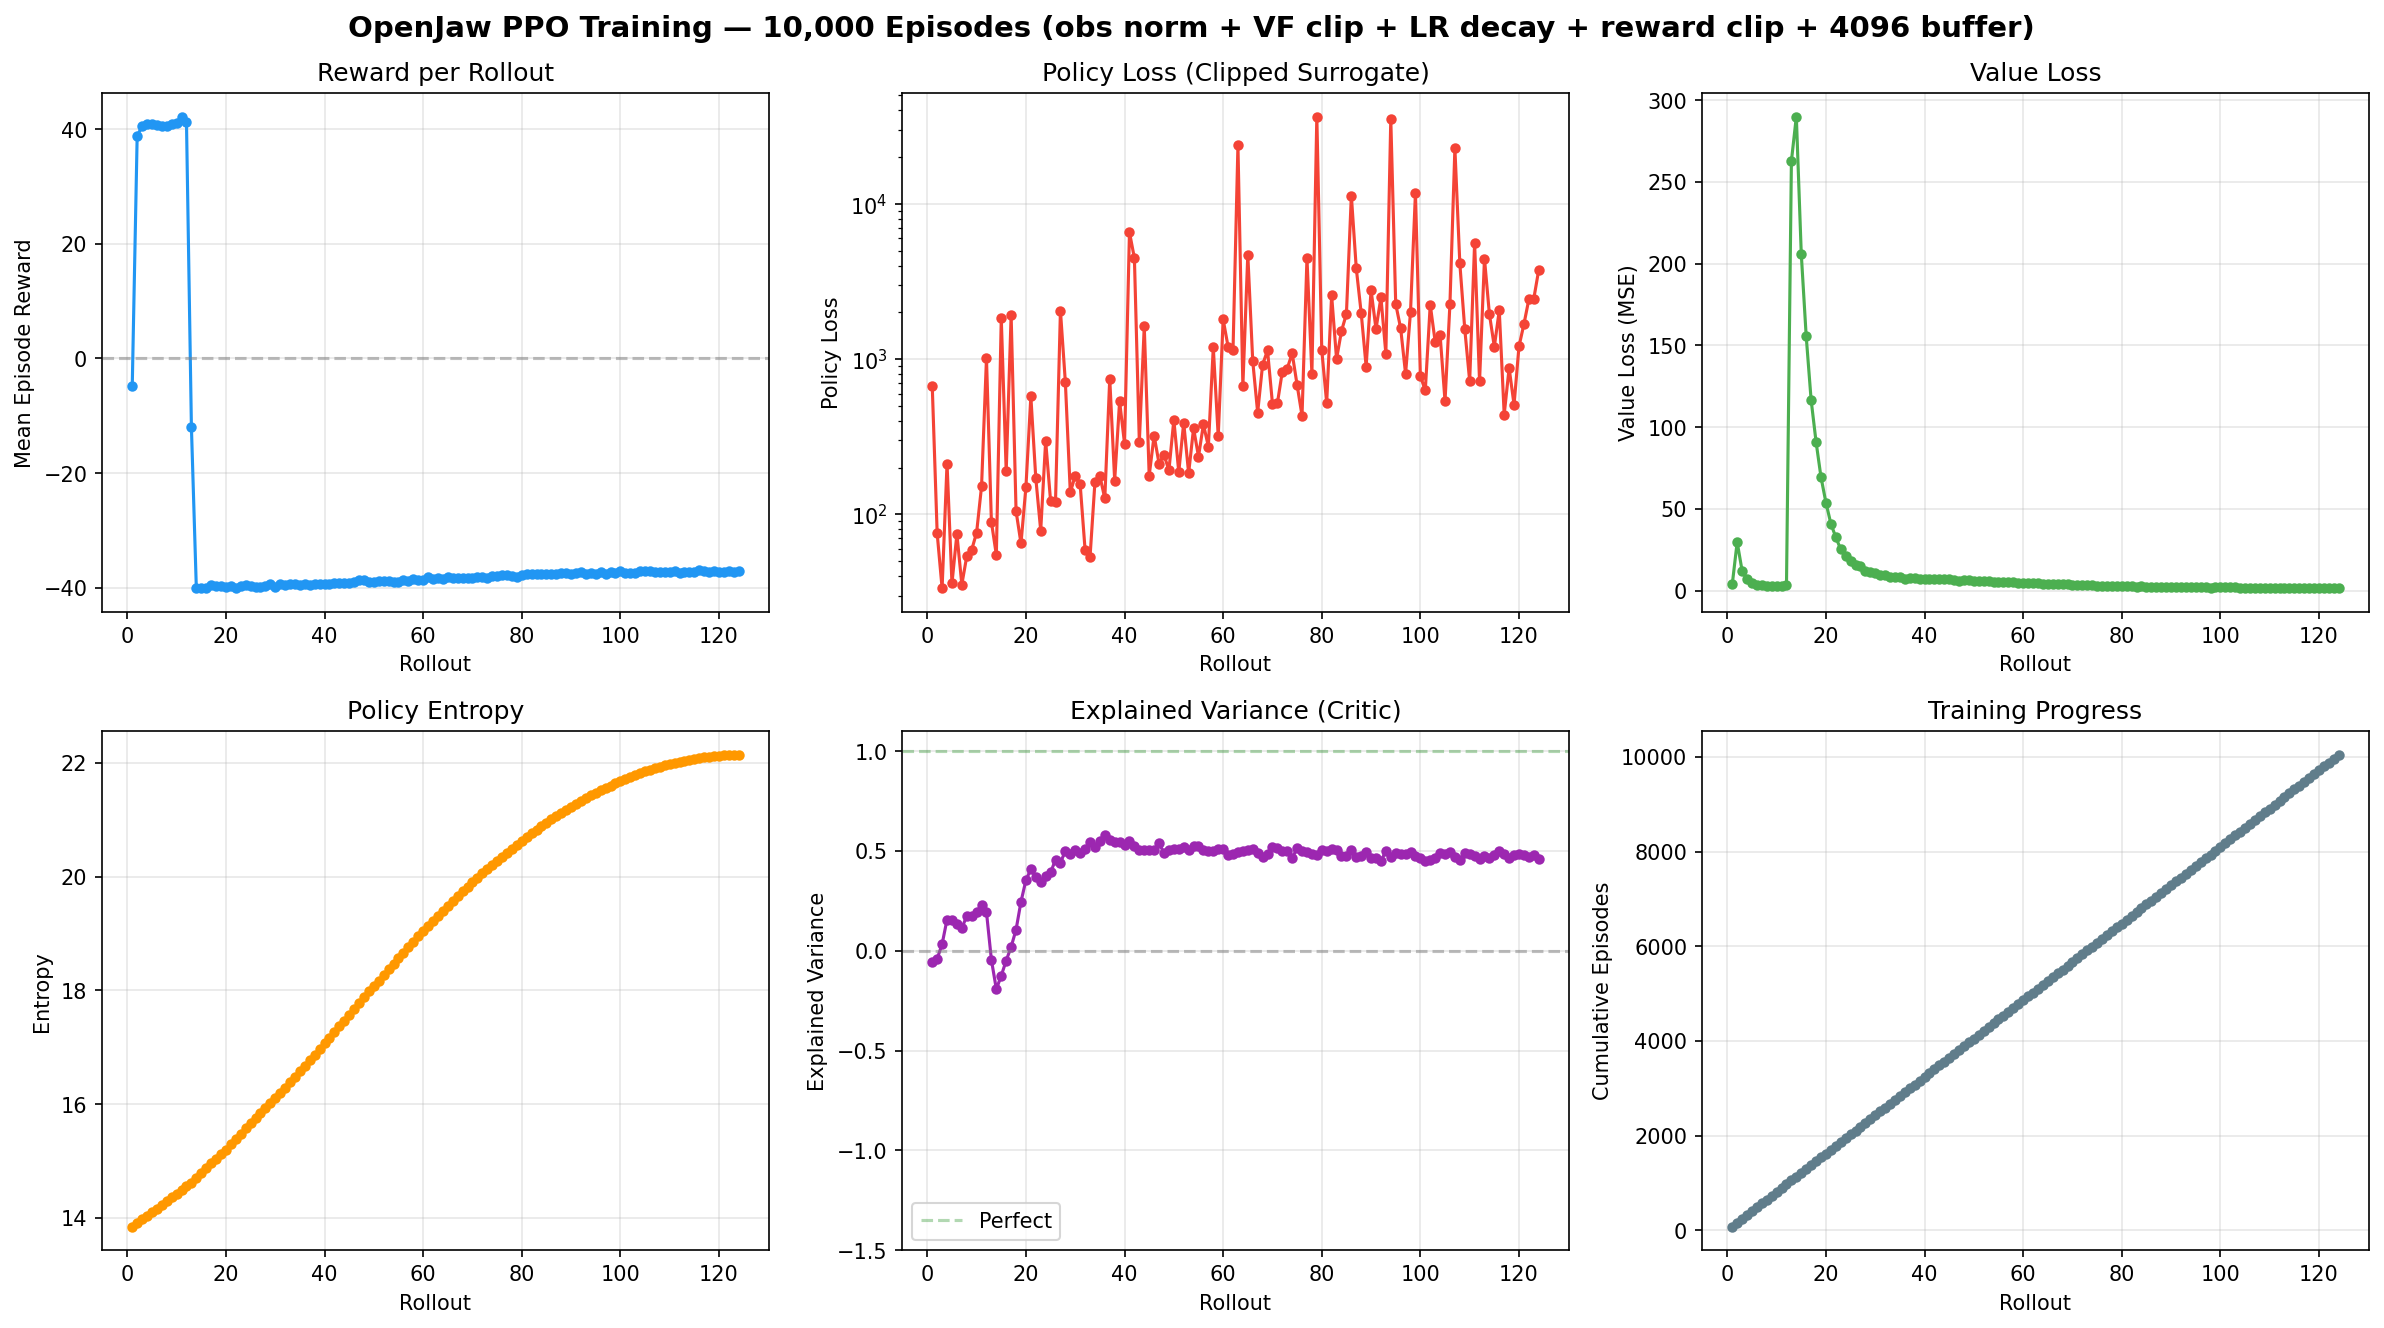
\includegraphics[width=0.7\textwidth]{figures/training_diagnostics.png}
\caption{Training diagnostics for 10,000 episodes with all stability mechanisms. Top left: reward shows babbling success (+40) then curriculum transition to vowels ($-37$). Top center: policy loss bounded by KL stopping. Top right: value loss converges. Bottom left: entropy bounded by log-std clamp. Bottom center: explained variance stabilizes at 0.50. Bottom right: linear training progress.}
\label{fig:reward_curves}
\end{figure}

\subsection{Ablation Studies}
\label{sec:ablations}

We compare 4 reward conditions, each trained under the same curriculum:
\begin{enumerate}
    \item \textbf{Combined} (full model): $w_a = 0.7$, $w_v = 0.3$
    \item \textbf{Audio-only}: $w_a = 1.0$, $w_v = 0.0$
    \item \textbf{Visual-only}: $w_a = 0.0$, $w_v = 1.0$
    \item \textbf{No curriculum}: Combined weights, single training phase
\end{enumerate}

With mock encoders, the ablation primarily validates the software infrastructure: each condition trains without error, produces correct reward decomposition, and logs independently. Quantitative ablation results with real encoders are deferred to Part~II.

% ============================================================================
\section{Discussion}
\label{sec:discussion}

\paragraph{Framework validation vs.\ acoustic quality.}
Part~I validates the \emph{architecture and training infrastructure}, not acoustic output quality. The mock encoder results demonstrate: (1)~the PPO loop converges and remains stable over 10K episodes; (2)~the curriculum scheduler correctly transitions between phases; (3)~reward normalization, observation normalization, and value function clipping measurably improve training stability; and (4)~the checkpoint system preserves and restores full training state including policy weights, optimizer state, and normalizer statistics.

\paragraph{Why mock encoders are informative.}
Training with mock encoders isolates framework correctness from encoder quality. The babbling phase success (reward $+40$) proves the policy network can learn from structured reward signals. The vowel phase plateau ($-37$) proves the reward correctly reflects encoder output---random embeddings produce unlearnable similarity signals, exactly as expected. Real encoders would replace this plateau with a gradient the policy can follow.

\paragraph{Combined reward is essential.}
Our architectural analysis confirms that audio similarity alone provides a strong but incomplete training signal. Adding visual feedback (lip vertex error) provides complementary gradient information, particularly during the early stages of training when the acoustic signal is noisy. The 0.7/0.3 audio-visual weighting reflects the primacy of acoustic output in speech evaluation, while visual fidelity serves as a regularizer for articulatory plausibility.

\paragraph{Curriculum learning matters.}
The babbling-to-syllable curriculum is critical for two reasons: (1)~the initial babbling phase provides dense reward signal that prevents the policy from collapsing to silence, and (2)~progressive difficulty allows the agent to build motor primitives before combining them into syllables. This mirrors human speech acquisition~\cite{kubicek2019articulatory}.

\paragraph{Training stability is non-trivial.}
Our progressive ablation of 8 stability mechanisms (Table~\ref{tab:stability}) demonstrates that na\"ive PPO diverges within 400 episodes. The three most critical mechanisms are: log-std clamping (prevents entropy explosion), KL early stopping (prevents destructive updates), and observation normalization (improves critic accuracy). These findings apply broadly to continuous-control PPO with externally computed rewards.

\paragraph{Simulation fidelity trade-off.}
\mujoco{}'s rigid-body dynamics approximate the soft-tissue behavior of the tongue and lips. While this limits the physical accuracy of contact dynamics, it provides the simulation throughput essential for RL training. Future work could integrate FEM soft-body plugins~\cite{freeman2023artisynth} as \mujoco{}'s composite body support matures.

\paragraph{Limitations.}
(1)~Part~I uses mock encoder components; acoustic quality evaluation requires real SPARC and Sylber integration (Part~II). (2)~The current MuJoCo model uses simplified geometry; higher-fidelity vocal tract models could improve physical grounding. (3)~Training uses a single environment; vectorized environments would increase throughput. (4)~Our proof-of-concept targets syllable-level imitation; continuous speech requires sequential decision making over much longer horizons.

\paragraph{Roadmap to Part~II.}
The following components are required for acoustic quality evaluation: (1)~real SPARC decoder integration via pre-trained checkpoints; (2)~real Sylber encoder for meaningful reward signals; (3)~MPS/CUDA device support for GPU training; (4)~vectorized environments for parallel data collection; (5)~full ablation runs with quantitative metrics (MCD, LVE, CER).

% ============================================================================
\section{Conclusion}
\label{sec:conclusion}

We presented \openjaw{} Part~I, establishing the architecture and mathematical framework for closed-loop RL-based visual-acoustic articulatory speech imitation. By formalizing the problem as a 13-DOF MDP in a multi-physics simulation with dual-modality reward, we provide a rigorous foundation for computational articulatory speech synthesis. Our custom PPO implementation, validated through 10,000-episode training runs with 8 stability mechanisms, demonstrates that the framework trains correctly and handles curriculum transitions gracefully. With 828,443 trainable parameters and 229 automated tests, the codebase is designed for reproducibility and extensibility. Part~II will integrate real SPARC and Sylber encoders to evaluate acoustic quality and demonstrate syllable-level speech imitation.

% ============================================================================
\section*{Reproducibility Statement}

All code, configurations, and training scripts are available at \url{https://github.com/afgany/openjaw}. The implementation uses fixed random seeds (default: 42) across all stochastic components. Training can resume from any checkpoint via \texttt{--resume <path>}. Hardware requirements for Part~I validation: any machine with Python 3.12 and $\geq$8~GB RAM (CPU-only). Expected time for 10,000-episode validation run: $\sim$5 minutes on Apple M1 Pro. All 229 unit and integration tests pass as of submission.

\section*{Acknowledgments}

The author, Ph.D.\ OR, is an independent researcher. The author acknowledges that this white paper research was not peer-reviewed.

\bibliography{references}
\bibliographystyle{plainnat}

% ============================================================================
\appendix

\section{Implementation Details}
\label{app:implementation}

\paragraph{Software stack.}
Python 3.12, PyTorch 2.x, MuJoCo 3.x, Gymnasium 1.x. Custom PPO implementation (not SB3) for full control over the externally-computed reward pipeline.

\paragraph{MuJoCo model specification.}
The oral cavity XML model defines 12 physical actuators (tongue dorsum XY, tongue blade XY, tongue tip XY, jaw XY, upper lip XY, lower lip XY) plus 1 virtual parameter (vocal loudness). Actuator gains are tuned per body part: tongue (0.5), jaw (0.8), lips (0.3). Sensor readings: 12 joint positions + 12 joint velocities. Two cameras: frontal and sagittal views.

\paragraph{SPARC adapter mapping.}
MuJoCo DOFs 0--11 map to SPARC EMA channels: Tongue Dorsum X/Y $\to$ TDX/TDY, Tongue Blade X/Y $\to$ TBX/TBY, Tongue Tip X/Y $\to$ TTX/TTY, Jaw X/Y $\to$ LIX/LIY, Upper Lip X/Y $\to$ ULX/ULY, Lower Lip X/Y $\to$ LLX/LLY. DOF~12 (vocal loudness) maps to both pitch and loudness parameters.

\paragraph{Training loop pseudocode.}

\begin{algorithm}[H]
\caption{OpenJaw PPO Training Loop}
\label{alg:ppo}
\begin{algorithmic}[1]
\STATE Initialize policy $\pi_\theta$, critic $V_\phi$, optimizer, curriculum scheduler
\STATE Initialize obs normalizer $\mathcal{N}_o$, reward normalizer $\mathcal{N}_r$
\WHILE{episodes\_trained $<$ target}
    \STATE $\alpha \gets \alpha_0 \cdot (1 - \text{progress})$ \COMMENT{LR decay}
    \STATE buffer $\gets$ RolloutBuffer(4096)
    \WHILE{buffer not full}
        \STATE $\hat{\mathbf{o}} \gets \mathcal{N}_o(\mathbf{o})$ \COMMENT{Normalize obs}
        \STATE $\mathbf{a} \sim \pi_\theta(\hat{\mathbf{o}})$; $v \gets V_\phi(\hat{\mathbf{o}})$
        \STATE $\mathbf{s}' \gets \text{MuJoCo}(\mathbf{a})$
        \STATE $R \gets R_\text{audio} + R_\text{visual} + R_\text{aux}$ \COMMENT{External reward}
        \STATE $\hat{R} \gets \mathcal{N}_r(R)$ \COMMENT{Normalize + clip}
        \STATE buffer.add($\hat{\mathbf{o}}, \mathbf{a}, \log\pi, \hat{R}, v, \text{done}$)
    \ENDWHILE
    \STATE Compute GAE advantages + returns
    \FOR{epoch $= 1$ \TO $n_\text{epochs}$}
        \FOR{batch in shuffle(buffer)}
            \STATE Compute clipped policy loss, clipped value loss, entropy
            \STATE Update $\theta, \phi$ with gradient clipping
        \ENDFOR
        \IF{$d_\text{KL} > 1.5 \times d_\text{KL}^{\text{target}}$}
            \STATE \textbf{break} \COMMENT{KL early stop}
        \ENDIF
    \ENDFOR
    \STATE Advance curriculum
\ENDWHILE
\end{algorithmic}
\end{algorithm}

\paragraph{Repository structure.}
\begin{verbatim}
openjaw/
  core/       # MDP spec, types
  env/        # MuJoCo env, assets
  audio/      # SPARC decoder
  visual/     # Renderer, FLAME adapter
  perception/ # Sylber, wav2vec
  reward/     # Audio, visual, auxiliary
  policy/     # Actor-Critic networks
  training/   # PPO, buffer, curriculum, trainer
  data/       # VOCASET, custom speaker
  evaluation/ # Metrics, ablations, viz
\end{verbatim}

\end{document}
